% !TEX encoding = UTF-8 Unicode
\documentclass[a4paper]{article}

\usepackage{color}
\usepackage{url}
\usepackage[T2A]{fontenc} % enable Cyrillic fonts
\usepackage[utf8]{inputenc} % make weird characters work
\usepackage{graphicx}
\usepackage{cite}
\usepackage{amsmath,calc}
\usepackage{mathtools}
\usepackage{colortbl}
\usepackage{tikz}
\usepackage{algorithm}
\usepackage{algpseudocode}

\usepackage[english,serbian]{babel}
%\usepackage[english,serbianc]{babel} %ukljuciti babel sa ovim opcijama, umesto gornjim, ukoliko se koristi cirilica

\usepackage[unicode]{hyperref}
\hypersetup{colorlinks,citecolor=green,filecolor=green,linkcolor=blue,urlcolor=blue}

\usepackage{listings}

%\newtheorem{primer}{Пример}[section] %ćirilični primer
\newtheorem{primer}{Primer}[section]

\definecolor{mygreen}{rgb}{0,0.6,0}
\definecolor{mygray}{rgb}{0.5,0.5,0.5}
\definecolor{mymauve}{rgb}{0.58,0,0.82}

\lstset{ 
  backgroundcolor=\color{white},   % choose the background color; you must add \usepackage{color} or \usepackage{xcolor}; should come as last argument
  basicstyle=\scriptsize\ttfamily,        % the size of the fonts that are used for the code
  breakatwhitespace=false,         % sets if automatic breaks should only happen at whitespace
  breaklines=true,                 % sets automatic line breaking
  captionpos=b,                    % sets the caption-position to bottom
  commentstyle=\color{mygreen},    % comment style
  deletekeywords={...},            % if you want to delete keywords from the given language
  escapeinside={\%*}{*)},          % if you want to add LaTeX within your code
  extendedchars=true,              % lets you use non-ASCII characters; for 8-bits encodings only, does not work with UTF-8
  firstnumber=1000,                % start line enumeration with line 1000
  frame=single,	                   % adds a frame around the code
  keepspaces=true,                 % keeps spaces in text, useful for keeping indentation of code (possibly needs columns=flexible)
  keywordstyle=\color{blue},       % keyword style
  language=Python,                 % the language of the code
  morekeywords={*,...},            % if you want to add more keywords to the set
  numbers=left,                    % where to put the line-numbers; possible values are (none, left, right)
  numbersep=5pt,                   % how far the line-numbers are from the code
  numberstyle=\tiny\color{mygray}, % the style that is used for the line-numbers
  rulecolor=\color{black},         % if not set, the frame-color may be changed on line-breaks within not-black text (e.g. comments (green here))
  showspaces=false,                % show spaces everywhere adding particular underscores; it overrides 'showstringspaces'
  showstringspaces=false,          % underline spaces within strings only
  showtabs=false,                  % show tabs within strings adding particular underscores
  stepnumber=2,                    % the step between two line-numbers. If it's 1, each line will be numbered
  stringstyle=\color{mymauve},     % string literal style
  tabsize=2,	                   % sets default tabsize to 2 spaces
  title=\lstname                   % show the filename of files included with \lstinputlisting; also try caption instead of title
}

\begin{document}

\title{Implementacija Sudoku rešavača korišćenjem Algoritma igrajućih pokazivača\\ \vspace{10px} \small{Seminarski rad u okviru kursa\\Konstrukcija i Analiza algoritama 2\\ Matematički fakultet}}

\author{Petar Đorđević}

%\date{9.~april 2015.}

\maketitle

\abstract{
  Ovaj rad istražuje Algoritam igrajućih pokazivača ({\em Dancing Links Algorithm - DLX}),
  koji je efikasna metoda za rešavanje problema pokrivanja tačaka, specifično za
  rešavanje problema tačnog omotača. Algoritam, koji je osmislio Donald
  Knut \cite{knuth}, omogućava brzu i efikasnu manipulaciju matrica
  pokrivanja. Ova tehnika je naročito pogodna za rešavanje složenih kombinatornih
  problema kao što je raspoređivanje poslova, logičke  rešetke, puzzle i slično.
  U okviru ovog rada, implementiraće se Sudoku rešavač kao konkretan primer primene 
  Algoritma igrajućih pokazivača (DLX).

\tableofcontents

\newpage

\section{Uvod}
Problem tačnog pokrivača ({\em Exact Cover Problem}) je klasičan kombinatorni problem odabira podskupova
iz date kolekcije tako da svaki element univerzalnog skupa bude tačno jednom pokriven \cite{cover}.
Rešavanje ovog problema ima primenu u raznim oblastima kao što su teorija grafova, optimizacija,
veštačka inteligencija i računarstvo. Problem tačnog pokrivača je NP-težak, što znači da je izuzetno
složen za rešavanje, te zahteva najbolji mogući algoritam za efikasno pronalaženje rešenja.

Jedan od najpoznatijih algoritama za rešavanje ovih problema je Algoritam igrajućih
pokazivača ({\em Dancing Links Algorithm - DLX}), koji je osmislio Donald Knuth. DLX
koristi strukturu podataka poznatu kao igrajući pokazivači koja optimizuje operacije
dodavanja, uklanjanja i pretraživanja elemenata u matricama pokrivanja.

Sudoku je popularna logička slagalica koja zahteva popunjavanje 9x9 mreže brojevima od 1 do 9,
uz poštovanje pravila da se svaki broj mora pojaviti tačno jednom u svakom redu, koloni i 3x3
podmreži. Problem rešavanja Sudokua može se preformulisati kao problem tačnih pokrivača, što ga
čini idealnim za primenu DLX-a. Ovo preformulisanje omogućava da se koristi DLX za efikasno
pronalaženje rešenja, čak i za najteže zagonetke.

Cilj ovog rada je da implementira Sudoku rešavač koristeći Algoritam igrajućih pokazivača i da
demonstrira efikasnost ovog algoritma. Pored toga, rad će evaluirati performanse DLX-a na
različitim primerima Sudoku zagonetki.

\section{Problem tačnog omotača}

Problem tačnog pokrivača ({\em Exact Cover Problem - ECP}) predstavlja ključnu podvrstu problema
zadovoljivosti ograničenja ({\em Constraint Satisfaction Problems - CSP}), gde je cilj
pronalaženje podskupa elemenata koji tačno pokrivaju dati skup. Svaki podskup se može posmatrati
kao klauza, a tačno pokrivanje zahteva da svaka klauza bude zadovoljena tačno jednom.

ECP se može definisati na sledeći način: Dat je univerzalni skup \( U \)
i kolekcija \( S \) podskupova \( U \). Cilj je pronaći podskup \( S' \subseteq S \) takav
da su svi elementi iz \( U \) tačno jednom pokriveni, odnosno svaki element iz \( U \) pripada
tačno jednom podskupu iz \( S' \).

\[
\mathcal{S}' \subseteq \mathcal{S} \quad \wedge \quad \left( \forall S_1, S_2 \in \mathcal{S}', \ S_1 \neq S_2 \implies S_1 \cap S_2 = \emptyset \right) \quad \wedge \quad \bigsqcup_{S' \in \mathcal{S}'} S' = U
\]

ECP se može svesti na CSP \cite{reduction} na sledeći način: \( S \) predstavlja izbore koje možemo
napraviti a \( U \) ograničenja nad tim izborima. Pošto je ova redukcija moguća  znamo da je to NP-težak problem.

Postoje različiti pristupi rešavanju ECP-a, među kojima su i algoritmi koji koriste tehniku pretraživanja
unazad, kao što su algoritam tačne pretrage i algoritam podeli pa vladaj. Pored toga, neki od najefikasnijih
algoritama za rešavanje problema tačnog pokrivača su bazirani na pretraživanju uz upotrebu heuristika, kao
što su gramzivi algoritmi i algoritmi zasnovani na tačnom pokrivanju kontraprimera ({\em backtracking}).
Ovi algoritmi kombinuju preciznost i efikasnost kako bi pronašli optimalna rešenja ili dobra približna rešenja
problema tačnog pokrivača.

\subsection{Matrica pokrivanja}

ECP se može predstaviti matricom incidencije: svaki red u matrici predstavlja jedan element iz skupa
\( S \) dok kolona predstavlja element iz skupa \( U \). U takvoj matrici, \( M_{ij} \) je \( 1 \)
ukoliko se element \( U_{j} \) nalazi u podskupu \( S_{i} \), a \( 0 \) obratno. ECP se rešava tako
što se ''uklone'' svi redovi tako da u svakoj koloni postoji tačno jedno polje koje ima vrednost \( 1 \).
U tabeli \ref{tab:incidencije} možete videti primer matrice incidencije za sledeći problem:\\
$$U = \{A, B, C, D, E, F, G\}$$
$$S = \{\{C, E, F\}, \{A, D, G\}, \{B, C, F\}, \{A, D\}, \{B, G\}, \{D, E, G\}\}$$
$$S' = \{\{C, E, F\}, \{A, D\}, \{B, G\}\}$$
\begin{table}[htbp]
  \centering
  \caption{Primer matrice incidencije}
  \label{tab:incidencije}
  \begin{tabular}{|c|*{7}{c|}}
    \hline
    A & B & C & D & E & F & G \\
    \hline
    \rowcolor{green} 0 & 0 & 1 & 0 & 1 & 1 & 0 \\
    1 & 0 & 0 & 1 & 0 & 0 & 1 \\
    0 & 1 & 1 & 0 & 0 & 1 & 0 \\
    \rowcolor{green} 1 & 0 & 0 & 1 & 0 & 0 & 0 \\
    \rowcolor{green} 0 & 1 & 0 & 0 & 0 & 0 & 1 \\
    0 & 0 & 0 & 1 & 1 & 0 & 1 \\
    \hline
  \end{tabular}
\end{table}

Ovakva matrica se zove matrica pokrivanja. Pretraga matrice pokrivanja za ECP često može biti spora zbog
činjenice da se moraju pretraživati sva polja matrice kako bi se pronašla ona koja sadrže 1. Kako se matrica
pokrivanja često sastoji od većeg broja redova i kolona, mnogo vremena se može potrošiti na pretragu polja
koja sadrže 0 pre nego što se dođe do onih koja sadrže 1. Ovo može usporiti izvršavanje algoritma za rešavanje
ECP-a, posebno u slučaju kada matrica pokrivanja ima velike dimenzije.

\section{Algoritam igrajućih pokazivača}

Algoritam igrajućih pokazivača ({\em Dancing Links Algorithm - DLX}), poznatiji kao ''Algoritam X'', je
efikasan algoritam, definisan od strane Donalda Knutha u radu objavljenom 2000. godine \cite{knuth},
koji se koristi za rešavanje ECS-a i sličnih kombinatornih problema. Ovaj algoritam koristi specifičnu
strukturu podataka nazvanu igrajući  pokazivači koja korišćenjem dvostruko povezanih listi optimizuje
operacija dodavanja, uklanjanja i pretraživanja elemenata u matricama pokrivanja. Zasnovana je na ideji
da se optimizuje pretraga matrice pokrivanja tako što se uvede matrica dvostruko uvezanih listi i time
eliminiše obilazak polja u matrici koja imaju vrednost \( 0 \).

\subsection{Operacije nad dvostruko ulančanim listama}

Neka je \( x \) pokazivač na element dvostruko ulančane liste. Takođe, neka \( L[x] \) i \( R[x] \)
predstavljaju pokazivač na element levo, odnosno desno od \( x \). Možemo definisati dve operacije:

\begin{minipage}{0.45\textwidth}
  \[
  \texttt{hide(x)} \vcentcolon =
  \begin{cases}
    L[R[x]] \gets L[x] \\
    R[L[x]] \gets R[x]
  \end{cases}
  \]
\end{minipage}
\begin{minipage}{0.45\textwidth}
  \[
  \texttt{unhide(x)} \vcentcolon =
  \begin{cases}
    L[R[x]] \gets x \\
    R[L[x]] \gets x
  \end{cases}
  \]
\end{minipage}


Operacija \( hide(x) \) uklanja element iz liste, dok ga \( unhide(x) \) vraća u listu ukoliko
je prethodno izbačen, a u suprotnom ne radi ništa. Uzastopno izvršavanje \( hide(x) \) pa \( unhide(x) \)
vraća listu u prvobitno stanje, i obe operacije su idempotentne (kod uzastopnih poziva iste operacije nad
istim elementom, samo prvi može promeniti listu, naredni pozivi ne rade ništa).

Usled gore navedenih osobina, dvostruko ulančane liste su pogodne za pamćenje stanja i simulaciju backtrackinga.

\subsection{Struktura igrajućih linkova}
Osnovna ideja ovog algoritma je korišćenje cikličnih dvostruko ulančanih listi kako bi se predstavila
matrica pokrivanja. Matrica se formira tako što se svaki red predstavlja jednim elementom koji treba
pokriti, a svaka kolona predstavlja jedan mogući način da se taj element pokrije. Cilj je da se odabere
kombinacija kolona (elementi) koja pokriva sve redove, pri čemu svaki element treba biti pokriven tačno
jednom. Svaki element u matrici je jedan čvor ciklične liste, a lista se formira ne samo po redovima već
i po kolonama tako da jedan element pripada zapravo dvema cikličnim dvostruko ulančanim listama: lista
kolone i lista vrste. Dodatno, matrica obično sadrži i red zaglavlja i cvor koren. Red zaglavlja se
koristi za identifikaciju kolona u matrici, dok se cvor koren koristi kao ulazna tačka u strukturu
podataka, omogućavajući jednostavan pristup početnim tačkama pretrage. Na slici \ref{fig:dlx} ilustrovano
je inicijalno stanje igrajućih linkova primera iz tabele \ref{tab:incidencije}.

\begin{figure}[h!]
  \begin{center}
  \includegraphics[scale=0.425]{slike/dlx.png}
  \end{center}
  \caption{Ilustacija inicijalnog stanja igrajućih linkova primera iz tabele \ref{tab:incidencije}}
  \label{fig:dlx}
\end{figure}

Jedan čvor u ovim listama se obično sastoji od pet polja:
\begin{itemize}
  \item \( L[x] \): Pokazivač na levi susedni čvor.
  \item \( R[x] \): Pokazivač na desni susedni čvor.
  \item \( U[x] \) : Pokazivač na gornji susedni čvor.
  \item \( D[x] \): Pokazivač na donji susedni čvor.
  \item \( C[x] \): Pokazivač na ''kolonu'' čvora, što predstavlja zaglavlje kolone u matrici.
\end{itemize}

Pored ovih polja, čvor unutar zaglavlja takođe ima i polje \( size[x] \) koje sadrži broj elemenata u
koloni, i polje \( name[x] \) koje sadrži labelu (ime) kolone. Ova polja nisu neophoda, ali pojednostavljuju
implementaciju strukture.

Algoritam DLX koristi backtracking strategiju, gde se prvo odabire jedan od mogućih elemenata (kolona) za
pokrivanje i proverava se da li je ova kombinacija valjana. Ako jeste, algoritam nastavlja dalje pretragu
u istom pravcu, inače se vraća korak unazad (backtrack) i bira drugi element za pokrivanje. Ovaj proces se
ponavlja sve dok se ne pronađe rešenje ili se iscrpe sve mogućnosti. Algoritam se izvodi rekurzivno
pretragom u dubinu kako bi se obišli svi mogući putevi u pretrazi.

\subsection{Operacije nad igrajućim pokazivačima}

Oslanjajući se na osobine funkcija  \( hide(x) \) i \( unhide(x) \) koje su malo pre definisane,
možemo slične funkcije definisati nad čvorovima tako da se mogu izvršavati i horizontalno i vertikalno.

Horizontalni slučaj:\\
\begin{minipage}{0.45\textwidth}
  \[
  \texttt{hideh(x)} \vcentcolon =
  \begin{cases}
    L[R[x]] \gets L[x] \\
    R[L[x]] \gets R[x]
  \end{cases}
  \]
\end{minipage}
\begin{minipage}{0.45\textwidth}
  \[
  \texttt{unhideh(x)} \vcentcolon =
  \begin{cases}
    L[R[x]] \gets x \\
    R[L[x]] \gets x
  \end{cases}
  \]
\end{minipage}\\

Vertikalni slučaj, proširen činjenicom da zaglavlje prati broj aktivnih elemenata u koloni:\\
  \begin{minipage}{0.45\textwidth}
  \[
  \texttt{hidev(x)} \vcentcolon =
  \begin{cases}
    U[D[x]] \gets U[x] \\
    D[U[x]] \gets D[x] \\
    C[x] \gets C[x] - 1
  \end{cases}
  \]
\end{minipage}
\begin{minipage}{0.45\textwidth}
  \[
  \texttt{unhidev(x)} \vcentcolon =
  \begin{cases}
    U[D[x]] \gets x \\
    D[U[x]] \gets x \\
    C[x] \gets C[x] + 1
  \end{cases}
  \]
  \end{minipage}\\

  Nakon što smo definisali osnovne operacije, možemo ih koristiti za implementaciju funkcija \texttt{cover} i
  \texttt{uncover}. Funkcija \texttt{cover(x)} sakriva kolonu \(x\) i sve redove koji je presecaju. Funkcija
  \texttt{uncover(x)} obnavlja kolonu \(x\) i sve redove koji je presecaju.

  \[
  \texttt{cover(x)} =
  \begin{cases}
  \texttt{hideh(x)} & \\
  \text{For } (\texttt{p} \gets \texttt{D[x]}; \quad \texttt{p} \neq \texttt{x}; \quad \texttt{p} \gets \texttt{D[p]}) & \\
  \quad \text{For } (\texttt{r} \gets \texttt{R[p]}; \quad \texttt{r} \neq \texttt{p}; \quad \texttt{r} \gets \texttt{R[r]}) & \\
  \quad \quad \texttt{hidev(r)} &
  \end{cases}
  \]
  
  Funkcija \texttt{cover(x)} prvo sakriva kolonu \(x\) pomoću \texttt{hideh(x)}. Zatim prolazi kroz sve redove ispod
  \(x\) koristeći pokazivač \texttt{p}. Unutar svakog reda, prolazi kroz sve desne elemente koristeći pokazivač
  \texttt{r} i sakriva ih pomoću \texttt{hidev(r)}.
  
  \[
  \texttt{uncover(x)} =
  \begin{cases}
  \text{For } (\texttt{p} \gets \texttt{U[x]}; \quad \texttt{p} \neq \texttt{x}; \quad \texttt{p} \gets \texttt{U[p]}) & \\
  \quad \text{For } (\texttt{l} \gets \texttt{L[p]}; \quad \texttt{l} \neq \texttt{p}; \quad \texttt{l} \gets \texttt{L[l]}) & \\
  \quad \quad \texttt{unhidev(l)} & \\
  \texttt{unhideh(x)} &
  \end{cases}
  \]
  
  Funkcija \texttt{uncover(x)} prvo prolazi kroz sve redove iznad \(x\) koristeći pokazivač \texttt{p}. Unutar svakog reda, prolazi kroz sve leve elemente koristeći pokazivač \texttt{l} i obnavlja ih pomoću \texttt{unhidev(l)}. Na kraju, obnavlja kolonu \(x\) pomoću \texttt{unhideh(x)}.

  Sada kada smo definisali osnovne operacije i funkcije \texttt{cover} i \texttt{uncover}, možemo preći na implementaciju samog DLX algoritma. Algoritam koristi rekurzivnu funkciju \texttt{search} koja pokušava da pronađe rešenje problema tačnog pokrivanja.

  \[
    \texttt{search(k)} =
    \begin{cases}
    \text{if } \texttt{R[head]} = \texttt{head} \\
    \quad \text{print solution and return} \\
    \text{else} \\
    \quad \texttt{c} \gets \text{choose column} \\
    \quad \texttt{cover(c)} \\
    \quad \text{For } (\texttt{r} \gets \texttt{D[c]}; \quad \texttt{r} \neq \texttt{c}; \quad \texttt{r} \gets \texttt{D[r]}) & \\
    \quad \quad \text{set solution[k] = r} \\
    \quad \quad \text{For } (\texttt{j} \gets \texttt{R[r]}; \quad \texttt{j} \neq \texttt{r}; \quad \texttt{j} \gets \texttt{R[j]}) & \\
    \quad \quad \quad \texttt{cover(j)} \\
    \quad \quad \texttt{search(k+1)} \\
    \quad \quad \text{For } (\texttt{j} \gets \texttt{L[r]}; \quad \texttt{j} \neq \texttt{r}; \quad \texttt{j} \gets \texttt{L[j]}) & \\
    \quad \quad \quad \texttt{uncover(j)} \\
    \quad \texttt{uncover(c)}
    \end{cases}
    \]

    Ova funkcija prvo proverava da li je problem rešen (ako je zaglavlje kolone jedino preostalo). Ako jeste, ispisuje rešenje i vraća se. Ako nije, bira se kolona \(c\) koja će biti pokrivena. Nakon što se kolona \(c\) pokrije, algoritam prolazi kroz sve redove \(r\) u toj koloni i pokušava da pronađe rešenje rekurzivnim pozivima funkcije \texttt{search(k+1)}. Ako se rešenje ne pronađe, kolone se otkrivaju kako bi se ispravile promene.

    Iako biranje kolone sa najmanjim brojem čvorova može delovati kao najefikasnija strategija za pokrivanje u algoritmu Igrajućih Linkova, često je korisno uvesti element pseudonasumičnosti u izbor kolone. Najčešća metoda je da se, u slučaju kada više kolona ima isti minimalni broj čvorova, izabere jedna kolona nasumično. Alternativno, može se implementirati potpuna pseudonasumičnost, gde se kolone biraju prema unapred definisanoj nasumičnoj strategiji.
\section{Sudoku}

Sudoku je logička igra brojevima koja se igra na mreži od 9x9 kvadrata. Mreža je podeljena u devet manjih kvadrata od 3x3,
zvanih "podmreže" ili "blokovi". Cilj igre je popuniti prazne kvadrate brojevima od 1 do 9, tako da svaki red, svaka kolona i
svaka podmreža sadrže sve brojeve od 1 do 9 bez ponavljanja. Igra počinje sa delimično popunjenom mrežom. Brojevi u početnom
rasporedu ne smeju se menjati.

Ograničenja za popunjavanje mreže:
\begin{enumerate}
  \item U svako polje se može upisati samo jedan broj
  \item Svaki broj se može pojaviti samo jednom u svakom redu
  \item Svaki broj se može pojaviti samo jednom u svakoj koloni
  \item Svaki broj se može pojaviti samo jednom u svakoj podmreži 3x3
\end{enumerate}

\subsection{Svođenje na problem tačnog pokrivača}

Sudoku tabla se može svesti na problem tačnog pokrivača \cite{sudoku}. Poenta je definisati ograničenja table kao
matricu pokrivanja. Pošto u svako polje može da se upiše jedan od 9 brojeva, a tabla ima 81 polje, matrica pokrivanja
ima 729 redova. Uslovi se u kolonama mogu upisati na naredni način:
\begin{enumerate}
  \item Svaki broj od 1 do 9 može se pojaviti samo jednom u svakom polju. To zahteva 81 uslov, po jedan za svako polje, kako bi se obezbedilo da ne postoje dva broja u istom polju.
  \item Svaki broj se mora pojaviti samo jednom u svakom redu. Ovo uvodi 81 uslov za sve redove.
  \item Svaki broj se mora pojaviti samo jednom u svakoj koloni. Takođe, ovo uvodi 81 uslov za sve kolone.
  \item Svaki broj se može pojaviti samo jednom u svakoj 3x3 podmreži. Ovo dodaje još 81 uslov za sve podmreže.
\end{enumerate}

Ukupno, tablica ograničenja je dimenzije 729x324 predstavljeno kao na slici \ref{fig:tabla}. 

\begin{figure}[h!]
  \begin{center}
  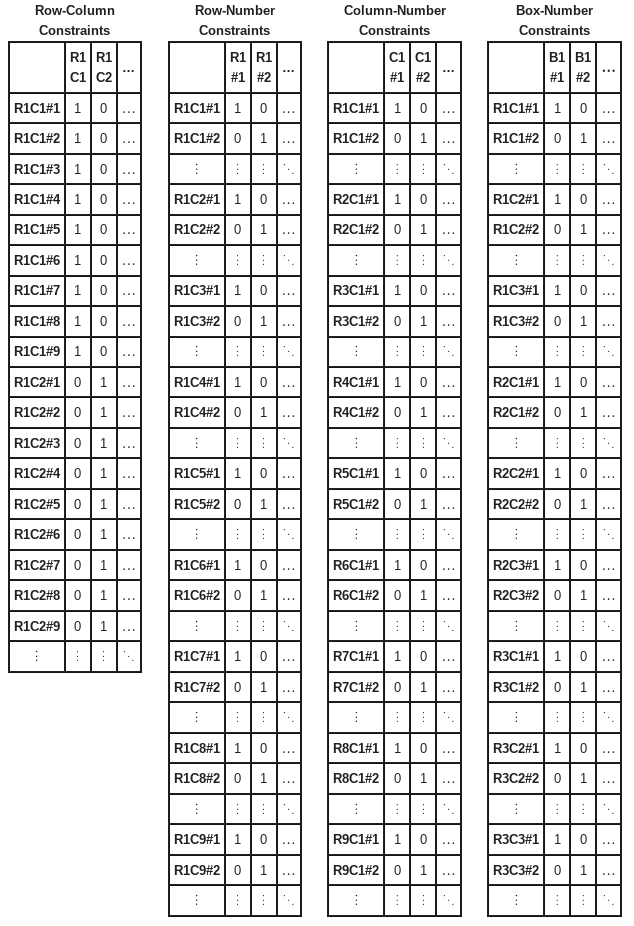
\includegraphics[scale=0.325]{slike/sudoku.png}
  \end{center}
  \caption{Definisanje uslova sudoku table preko matrice pokrivanja}
  \label{fig:tabla}
\end{figure}


\section{Zaključak}
\label{sec:zakljucak}

U ovom radu istražena je primena Algoritma igrajućih pokazivača (DLX) u rešavanju problema tačnog pokrivača (ECP), s posebnim fokusom
na popularnu logičku igru Sudoku. Proučena je struktura matrice pokrivanja i njeno preformulisanje u kontekstu Sudoku igre, što je
omogućilo efikasno korišćenje DLX algoritma za pronalaženje rešenja.

Primena DLX algoritma na Sudoku problem pokazala je značajnu efikasnost u rešavanju kompleksnih zagonetki, zahvaljujući optimizaciji
pretrage matrice pokrivanja kroz strukturu dvostruko ulančanih listi. Implementacija DLX-a demonstrira njegovu sposobnost da značajno
poboljša performanse u poređenju sa tradicionalnim metodama rešavanja Sudoku zagonetki, naročito u slučajevima sa velikim brojem praznih
polja.

Analizom rezultata, primećeno je da DLX ne samo da ubrzava proces rešavanja, već i smanjuje potrebu za memorijskim resursima, što je od
ključne važnosti za rad sa velikim instancama problema. Efikasnost algoritma dodatno je poboljšana primenom heurističkih metoda za izbor
kolona, čime je omogućeno da se pronalaženje rešenja postigne brže i sa manjim brojem pokušaja.

Ovaj rad doprinosi razumevanju kako napredni algoritmi za rešavanje kombinatornih problema mogu biti primenjeni u praksi, pružajući čvrstu
osnovu za buduće istraživanje u oblasti algoritamske optimizacije i rešavanja problema sa velikim dimenzijama.

Za buduće radove, preporučuje se istraživanje proširenja DLX algoritma na druge kombinatorne probleme i adaptaciju metodologije za rad sa
specijalizovanim strukturama podataka koje mogu dalje poboljšati efikasnost i primenljivost algoritma. Takođe, analiza različitih
heurističkih pristupa za izbor kolona može pružiti dodatne uvide u optimizaciju performansi DLX-a.

U zaključku, ovaj rad potvrđuje potencijal Algoritma igrajućih pokazivača kao moćan alat za rešavanje problema tačnog pokrivača i sličnih
kombinatornih problema, s velikim mogućnostima za primenu u različitim oblastima istraživanja i praktične primene.

\addcontentsline{toc}{section}{Literatura}
\bibliography{seminarski} 
\bibliographystyle{plain}



\end{document}
